\documentclass{article}
\usepackage[utf8]{inputenc}
\usepackage[space]{xeCJK}
\usepackage{amsmath}
\usepackage{esint}
\title{车尾识别与车辆控制}
\author{517030910314 顾诗轩}
\date{JUNE 2019}
\begin{document}
\maketitle
\tableofcontents
\newpage
\section{图像识别}
该方法是将车辆特征用相应的描述子来表示,然后用机器学习方法训练样本。
\newline\newline
目前,应用在车辆上的机器学习算法主要包括:Haar-like+Adaboost、HOG+SVM、HOG+Adaboost、HOG +Haar-like +Adaboost、阴影特征+Adaboost等方法。
\newline\newline
在基于机器视觉的车辆识别方法中,机器学习的识别方法由于具有良好的鲁棒性和优越的识别性能,使其越来越多地被应用于车辆识别当中。考虑到机器学习方法的优越性,本文使用基于Haar-like特征和Adaboost分类器的算法来对前方运动车辆进行识别。
\newline\newline
分类器的生成主要步骤为:利用类Haar特征从海量的车辆样本中提取相关特征,首先使用类Haar特征构建弱分类器,并通过Adaboost算法把弱分类器提升成为强分类器,然后把多个强分类器串联成级联分类器,得到最终的分类器。
\subsection{特征提取}
在提取Haar-like特征的部分,我们使用了积分图的计算进行操作。积分图就是只遍历一次图像就可以求出图像中所有区域像素和的快速算法,大大的提高了图像特征值计算的效率。
\newline\newline
积分图主要的思想是将图像从起点开始到各个点所形成的矩形区域像素之和作为一个数组的元素保存在内存中,当要计算某个区域的像素和时可以直接索引数组的元素,不用重新计算这个区域的像素和,从而加快了计算(这有个相应的称呼,叫做动态规划算法)。积分图能够在多种尺度下,使用相同的时间(常数时间)来计算不同的特征,因此大大提高了检测速度。
\newline\newline
大小为w×h的图像 f (x, y) 所对应的积分图像ii(a,b) 大小也为w×h 。如图所示,积分图像中每一个点 (a,b)的值是图像 f (x, y) 中从原点 (0,0) 到点(a,b) 所构成的矩形内部所有像素之和。积分图像的数学表达式如下:$$i i(a, b)=\sum_{x \leq a, y \leq b} I(x, y)$$
\newline
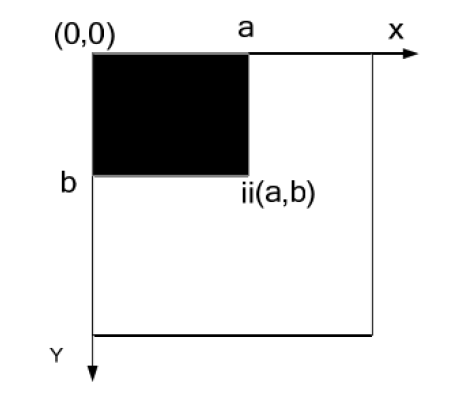
\includegraphics[scale=0.4]{ig.png}
\subsection{分类器建立}
分类器的建立首先从弱分类器开始实现,弱分类器是指分类正确率略大于50%的分类器,虽然具有结构简单、计算量小和实时性好等优点,但其分类能力较弱。本文中构建弱分类器的方法为:每一个 Haar 特征对应构建一个弱分类器。假设第 j 个 Haar 特征的特征值为 $f (x)_j$ ,则由该特征生成的弱分类器为:
$$h_{j}(x)=\left\{\begin{array}{l}{1, p_{j} f_{j}(x)<p_{j} \theta_{j}} \\ {0, \text { otherwise }}\end{array}\right.$$
其中,$h (x)_j$ 为弱分类器的分类结果,1表示车辆目标,0表示非车辆目标;j和p为不等式的方向参数,取值为1或-1,1表示不等式符号为小于号,-1表示不等式符号为大于号; j和θ 为弱分类器$h (x)_j$的阈值。构建基于类Haar特征的弱分类器,实际上是选择一个合适的特征值作为阈值,使得该分类器对于整个训练样本集中的样本分类错误率最低。当分类器有最小分类错误率时,其对应的类Haar 特征和特征值构成最佳组合,此时的特征值就是最合适的阈值。
\newline\newline
接着用Adaboost 算法实现强分类器的构建,主要是在训练过程中动态修改各样本的权重,更多地重视其中难以识别的样本。Adaboost算法首先是进行初始化,赋予同类训练样本以相同的权重。然后才开始对训练样本进行训练,假设共需要进行T轮训练。在每一轮训练结束后,都要在降低正确分类本权重的同时,增加错误分类样本权重,从而在下次训练时更多地重视错误分类样本。在T 轮训练结束后,将获得的T 个弱分类器加权组合成强分类器,最后再用得到的强分类器。具体步骤如下:
\newline\newline
首先进行样本集准备。假设容量为 n 的样本集:$\left\{\left(x_{1}, y_{1}\right), \ldots\left(x_{i}, y_{i}\right), \ldots,\left(x_{n}, y_{n}\right)\right\}$其中,n 为样本总数;$x_i$表示第i个样本的特征向量;$y_i$表示第i个样本的标签,若是正样本记为1,负样本则记为0。假设样本集中共有l个正样本,m 个负样本,$l +m = n$,每个样本共有k个类Haar 特征。
\newline\newline
接着进行初始化权重。当 $y_i=0$ 时为负样本:$$w_{1, i}=\frac{1}{2 m}$$当 $y_i=1$ 时为正样本:$$w_{1, i}=\frac{1}{2 l}$$式中,$w_{1,i}$ 为第一轮训练中第i 个样本对应的权重。
\newline\newline
最后进行权重归一化:$$w_{t, i}=\frac{w_{t, i}}{\sum_{i=1}^{n} w_{t, i}}, i=1,2, \ldots, n$$
对于第j 个特征, 根据给定权重训练弱分类器$h_{t,j}$, ,并计算其相对于当前权重的误差$ε_{t,i}$;$$\varepsilon_{t, i}=\sum_{i=1}^{n} w_{t, i}\left|h_{t, i}\left(x_{i}\right)-y_{i}\right|$$
$$h_{t, j}=\left\{\begin{array}{l}{1, p_{j} f_{j}<p_{j} \theta_{j}} \\ {0, \text { OTHERS }}\end{array}\right.$$
$$j=1,2, \ldots k$$
式中, $h_{t,j}$ , 为弱分类器的值; $f_j$为第j 个特征的特征值; $\theta_j$为阈值;$ p_j∈{−1,1} $,表示分类方向。
\newline\newline
然后更新每个样本所对应的权重:$$\mathcal{W}_{t+1, i}=w_{t, i} \beta_{t}^{1-e_{i}}$$
式中:$\beta_{t}=\varepsilon_{t} /\left(1-\varepsilon_{t}\right)$;若样本$x_i$被正确分类,则 $e_i=0$ ;否则,$e_i=1$。
生成的强分类器如下:
$$h(x)=\left\{\begin{array}{l}{1, \sum_{t=1}^{T} \alpha_{t} h_{t}(x) \geq \frac{1}{2} \sum_{t=1}^{T} \alpha_{t}} \\ {0,Others}\end{array}\right.$$
\section{巡线仿真}
智能车的感知部分我们完成了车尾识别与测距的实现,为了提高本项目的完整性,我们还就智能车的车辆控制部分进行了巡线仿真。
\newline\newline
具体算法设计如下:
\newline
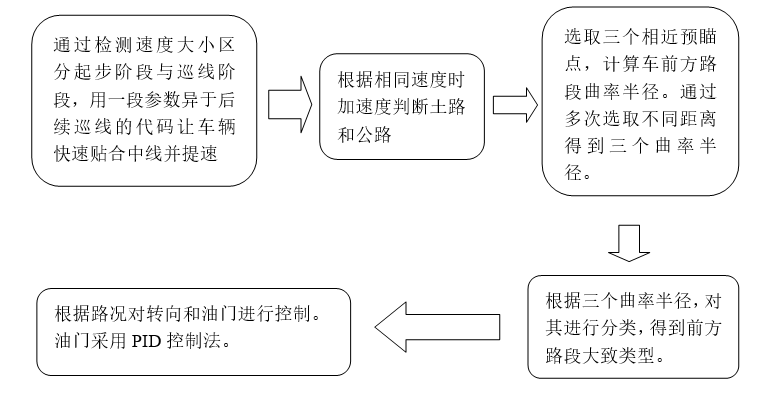
\includegraphics[scale=0.5]{cc.png}
\\代码部分在文件中已经给出,在此不做赘述。
\newline\newline
控制部分的核心算法中我们主要使用了PID,即比例积分微分控制,它是一种经典的反馈控制算法,其原理如下:
\newline 
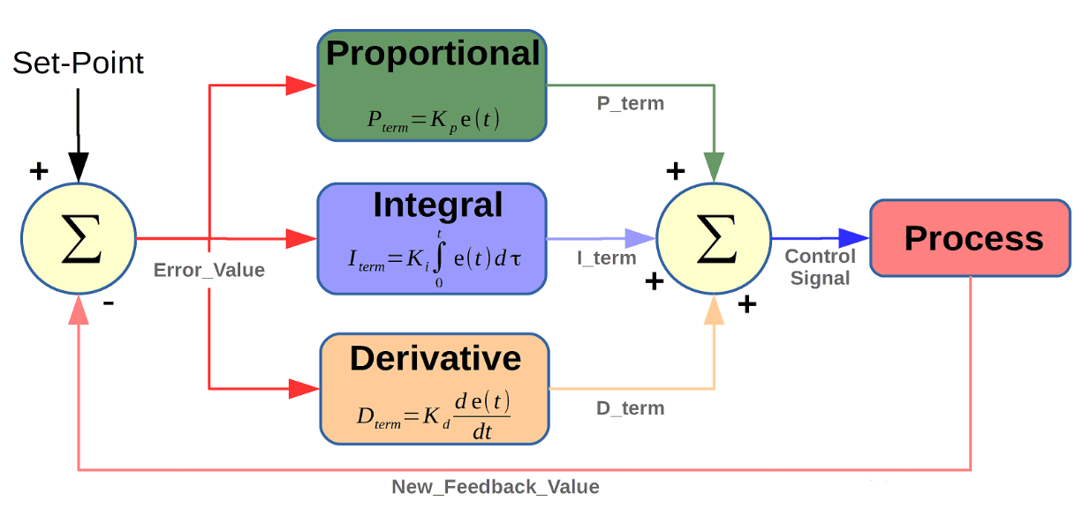
\includegraphics[scale=0.5]{pid.png}
\newline
数学表达式如下:
\newline
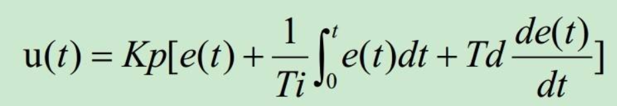
\includegraphics[scale=0.5]{PID2.png}
\newline\newline
就仿真部分而言,我们使用了CyberTORCS仿真平台进行测试,测试过程中我们使用了六种不同的路段赛道来比较,实验结果(时间单位)如下:
\newline
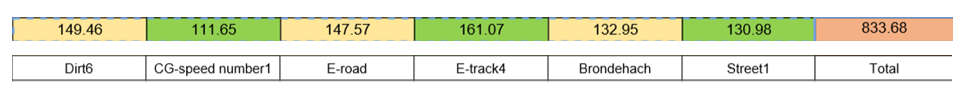
\includegraphics[scale=0.4]{res.png}
\newline\newline
仿真过程在展示中已经给出,在此给出部分截图
\newline
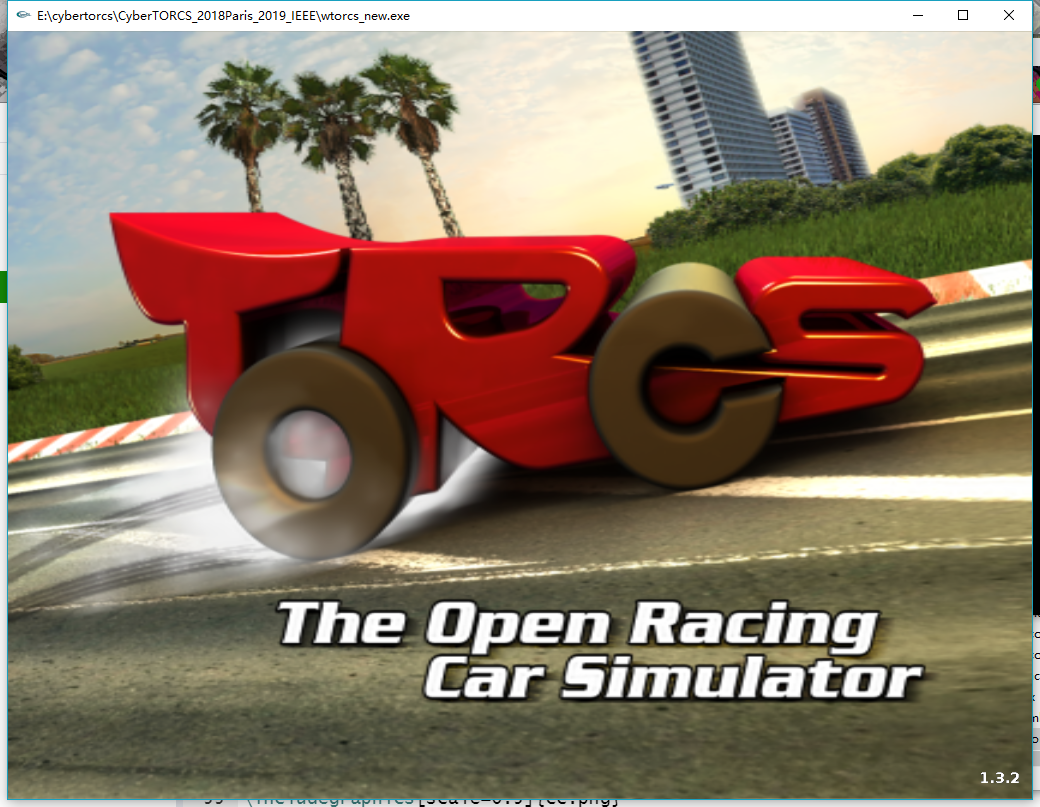
\includegraphics[scale=0.3]{t1.png}
\newline
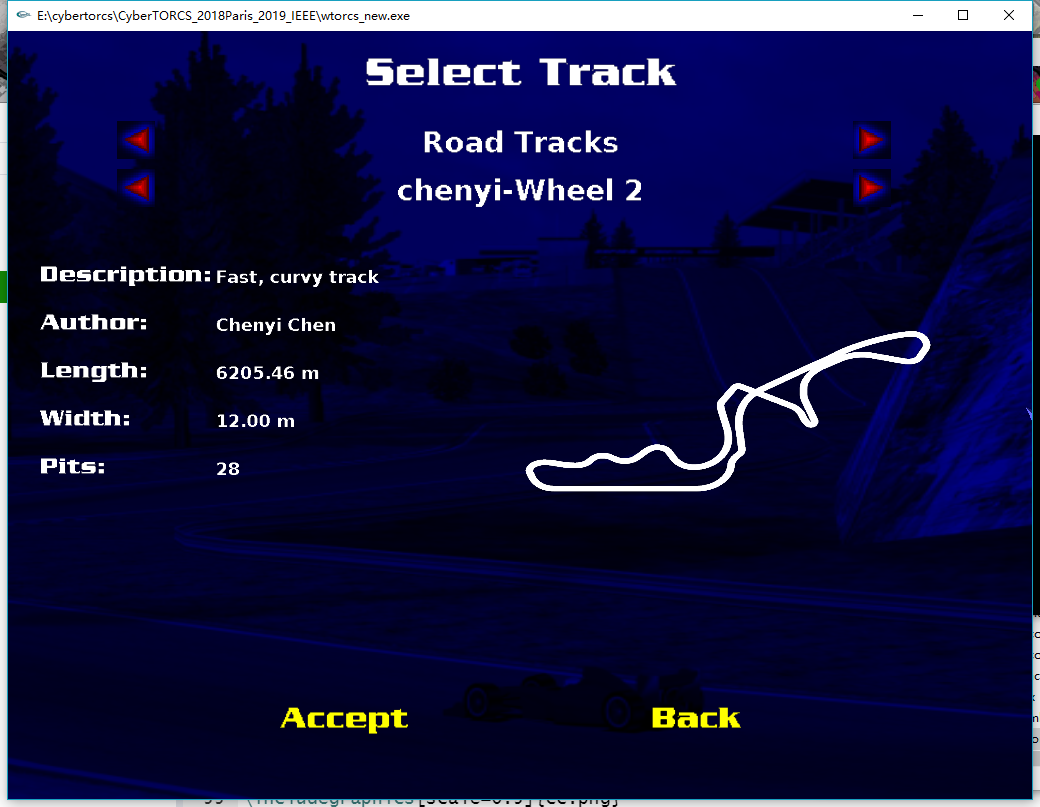
\includegraphics[scale=0.3]{t2.png}
\newline
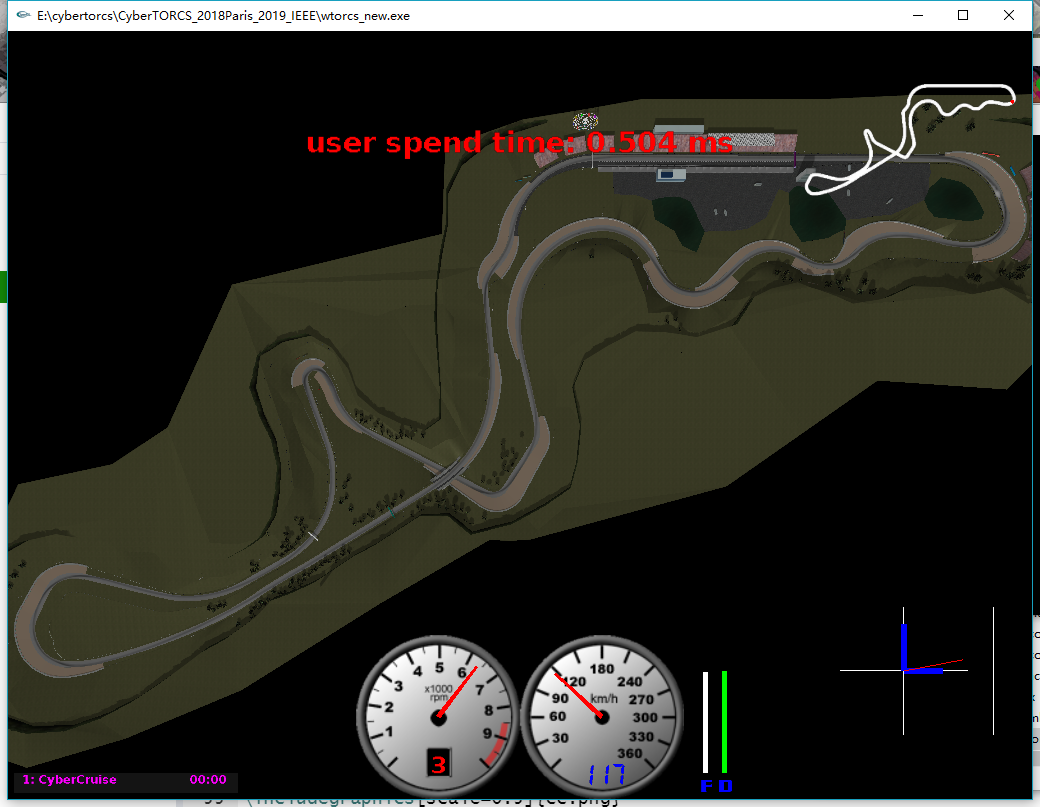
\includegraphics[scale=0.3]{t3.png}
\newline
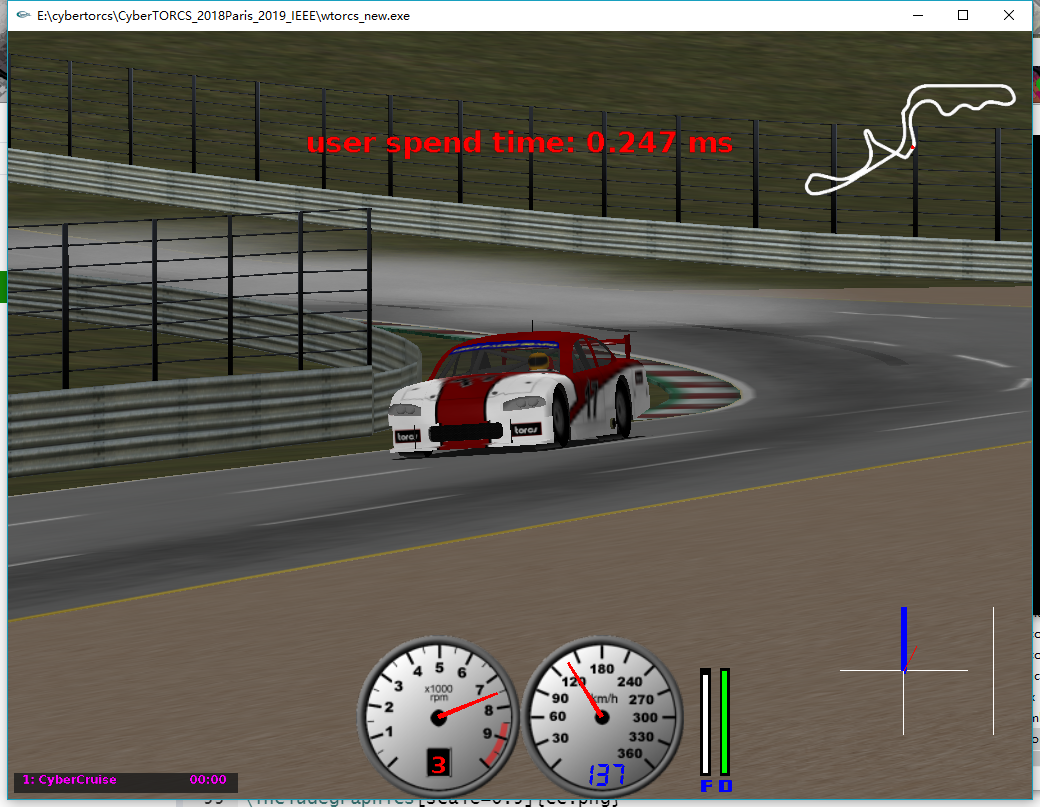
\includegraphics[scale=0.3]{t4.png}
\newline
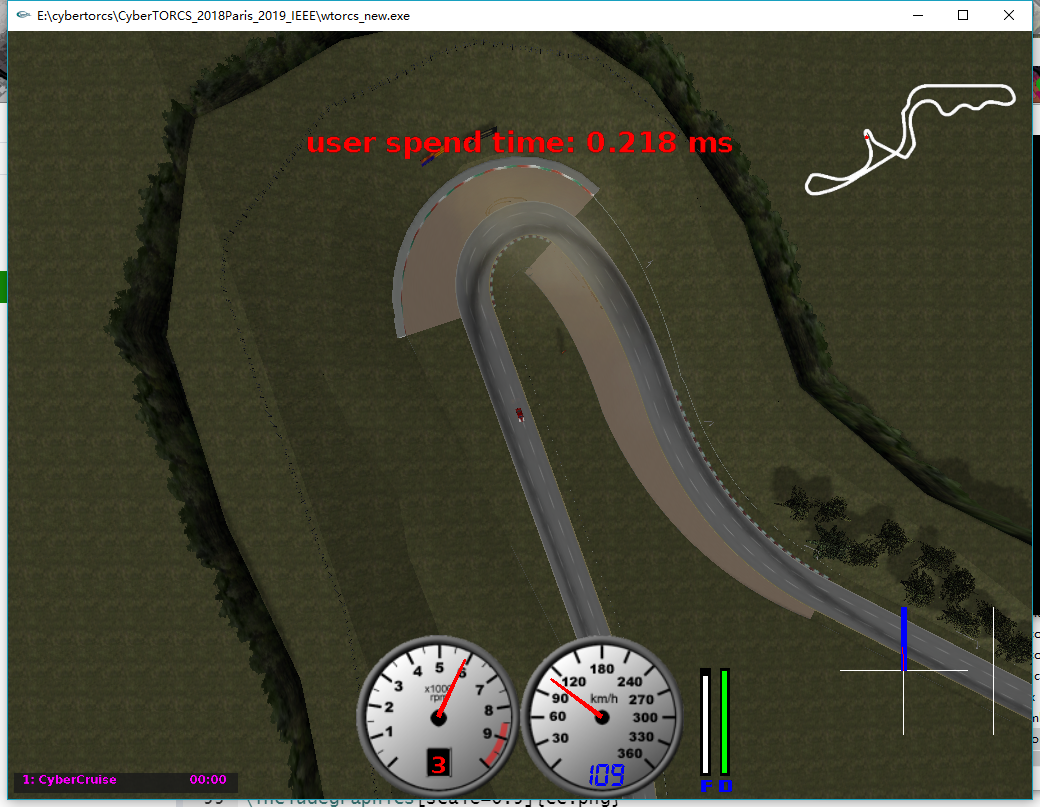
\includegraphics[scale=0.3]{t5.png}
\end{document}
